\section{Methodology and Pipeline Structure}

\subsection{Pipeline Architecture}

\begin{figure}[htbp]
    \centering
    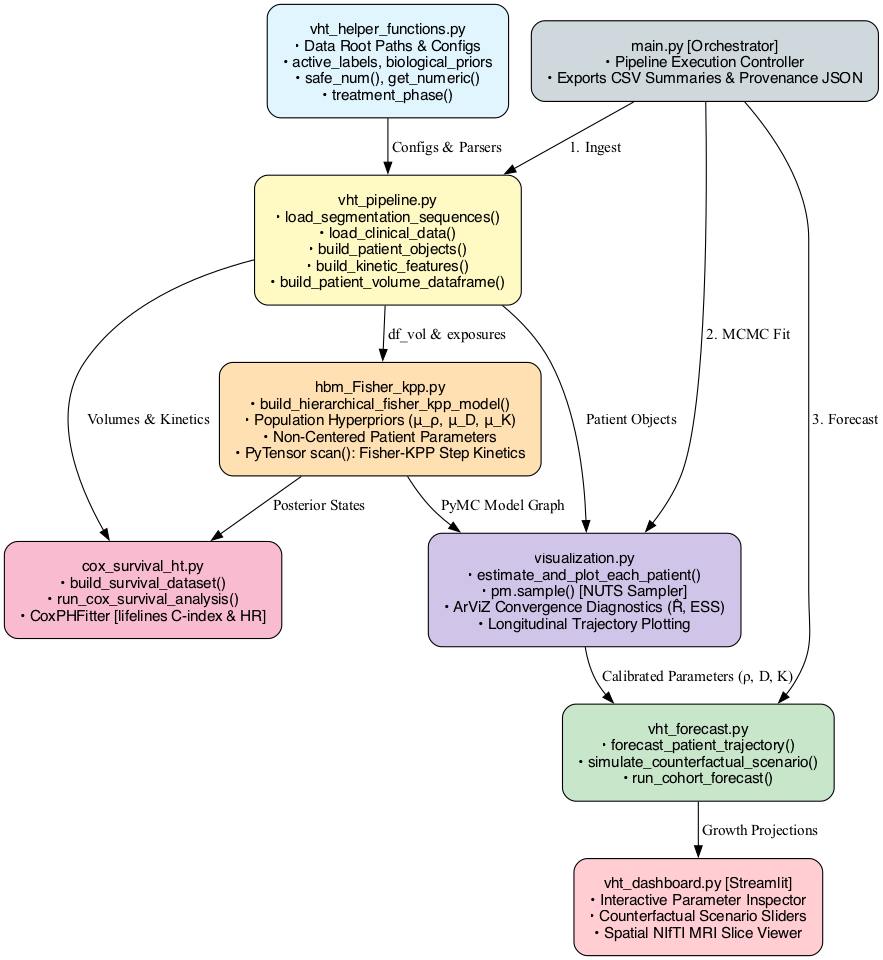
\includegraphics[width=0.85\textwidth]{figures/system_structure.png}
    \caption{Comprehensive structural architecture and module interaction flow of the NEXUS Brain Virtual Health Twin (VHT) framework.}
    \label{fig:system_structure}
\end{figure}

The \textsc{Nexus Brain} Virtual Health Twin (VHT) framework establishes an end to end computational pipeline for patient specific modeling of Glioblastoma progression. It integrates longitudinal Neuroimaging segmentations, multi center clinical histories, Radiobiological treatment parameters, and molecular biomarkers into a unified analytical workflow. The pipeline ingests multimodal MRI scans and clinical records through \texttt{vht\_pipeline.py}, extracting longitudinal tumor volumes, volumetric changes, and treatment exposure fractions. Rather than representing therapies as binary exposures, the framework quantifies the proportion of each inter scan interval during which Chemotherapy, Radiotherapy, Immunotherapy, additional therapies, or Brachytherapy was active.

These longitudinal imaging and treatment features are used to calibrate a Hierarchical Bayesian Model (HBM) implemented with \texttt{PyMC} and \texttt{PyTensor} in \texttt{hbm\_Fisher\_kpp.py}. The model is based on the Fisher-KPP Reaction Diffusion equation and estimates patient specific proliferation (\(\rho\)), diffusion (\(D\)), carrying capacity (\(K\)), and treatment efficacy coefficients (\(\alpha_m\)). The hierarchical structure enables the framework to capture both cohort level tumor growth patterns and individual deviations, allowing tumor dynamics of each patient to be represented by calibrated parameters informed by their own longitudinal data.

The calibrated parameters are subsequently passed to a forecasting and counterfactual simulation module, \texttt{vht\_forecast.py}. This module projects future tumor growth from the most recent available scan and evaluates hypothetical clinical scenarios by including surgical resection, altered treatment timing, and multi modal therapy schedules. Furthermore, by comparing projected trajectories under different assumptions, the framework supports “what-if” analyses of interventions that were not observed in the original clinical course.

The framework also provides interactive clinical exploration through a \texttt{Streamlit} dashboard, \texttt{vht\_dashboard.py}. The dashboard enables selection of individual patients, inspection of calibrated growth parameters and historical tumor volumes, configuration of virtual treatment scenarios, and visualization of projected tumor trajectories alongside longitudinal MRI data. Finally, \texttt{cox\_survival\_ht.py} links model derived tumor kinetics, treatment exposures, and genetic biomarkers to survival outcomes using regularized Cox proportional hazards modeling. Automated provenance logging through \texttt{run\_metadata.json} records key execution details, supporting transparency, reproducibility, and computational auditability across the full pipeline.





\subsection{Shared Configuration and Utility Functions (\texttt{vht\_helper\_functions.py})}

\begin{figure}[htbp]
    \centering
    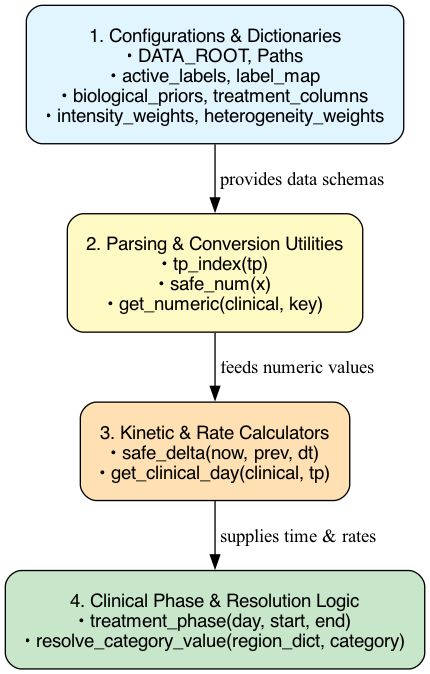
\includegraphics[width=0.35\textwidth]{figures/helper_functions_structure.png}
    \caption{Comprehensive structural architecture and module interaction flow of the NEXUS Brain Virtual Health Twin (VHT) framework.}
    \label{fig:helper_function_structure}
\end{figure}

The \texttt{vht\_helper\_functions.py} module provides the shared configuration, data mappings, and utility functions used throughout the \texttt{Nexus Brain} VHT pipeline. It standardizes the interpretation of raw clinical, imaging, and segmentation data before feature extraction, Bayesian calibration, forecasting, and survival modeling. By centralizing these operations, the module ensures consistent handling of tumor labels, clinical variables, treatment intervals, and derived imaging features. The module defines the locations of the primary data sources, including the MRI image directory, segmentation volume spreadsheet, and clinical data spreadsheet. It also specifies the clinical worksheet containing patient level records. Centralizing these paths ensures that downstream modules access the same source data and reduces the risk of inconsistent file handling.

Segmentation labels are harmonized into four biologically meaningful tumor compartments: necrotic core, enhancing tumor, edema, and resection cavity. Raw labels, such as "Necrotic Tumor Core (Label1)" and "Tumor Infiltration and Edema," are mapped to standardized categories. This harmonization is necessary because source data may use different naming conventions, while downstream modeling requires a consistent set of tumor subregions. Then module defines biological priors and treatment related clinical variables. Biological priors include established Glioblastoma associated molecular and genetic markers, such as \textit{IDH1} and \textit{IDH2} mutation, \textit{MGMT} promoter Methylation, \textit{1p/19q} codeletion, \textit{ATRX} mutation, \textit{TERT} promoter mutation, \textit{EGFR} amplification, \textit{PTEN} mutation, \textit{CDKN2A/B} deletion, \textit{TP53} alteration, and tumor grade. These variables are retained for downstream survival modeling and will be used to assess associations between molecular features, tumor kinetics, and clinical outcomes.

Treatment variables capture the type, timing, dose, and duration of Chemotherapy, Radiotherapy, additional systemic therapies, Immunotherapy, and Brachytherapy. Also this module defines paired Start and End day fields for each treatment type and allow the pipeline to construct treatment intervals relative to the date of diagnosis. It is essential for calculating treatment exposure during each MRI interval. Furthermore, this module defines modality specific weights for calculating composite intensity and heterogeneity features within each tumor compartment. Four MRI sequences are considered: contrast enhanced T1 weighted imaging (T1C), non contrast T1 weighted imaging (T1N), T2-FLAIR (T2F), and T2 weighted imaging (T2W). The weights reflect the expected relative contribution of each sequence to the biological interpretation of a given tumor region. For example, enhancing tumor regions are weighted most heavily toward T1C signal, because contrast enhancement is primarily associated with blood brain barrier disruption and active tumor tissue\cite{fan2024radiomics}. In contrast, edema is weighted more strongly toward T2-FLAIR and T2-weighted sequences, which are more sensitive to vasogenic edema and infiltrative change. Similar region-specific weighting is applied to heterogeneity features, enabling standardized measures of signal intensity and intratumoral variability across MRI sequences.

Several helper functions standardize the extraction of numeric values from heterogeneous clinical data. The \texttt{safe\_num()} function converts numeric values, numeric strings, and strings containing embedded numbers into floating point values. For example, a dose recorded as "60 Gy" or a fraction count recorded as "30 fractions" can be converted to 60.0 and 30.0, respectively. Missing, non numeric, or malformed entries are returned as \texttt{NaN}, preventing invalid values from entering the modeling pipeline. The \texttt{get\_numeric()} function extends this behavior for clinical metadata dictionaries. It performs robust key matching, removes unnecessary whitespace, recognizes common missing value labels such as "NA", "N/A" and "NONE", and extracts the first numeric value from mixed text number fields. This is particularly important for multi center clinical datasets, where the same variable may be recorded using different formats or units.

The \texttt{safe\_delta()} function calculates the rate of change of a variable between consecutive time points. It divides the difference between the current and previous value by the elapsed time while explicitly handling missing values and non positive time intervals. This function is used to derive features such as tumor volume velocity, voxel count velocity, and changes in image derived intensity or heterogeneity measures. The \texttt{get\_clinical\_day()} function maps each imaging time point to its corresponding number of days from diagnosis. It identifies clinical fields containing the relevant time point identifier and converts the associated value to a numeric day. This enables alignment of MRI derived tumor measurements with treatment windows and supports calculation of inter-scan time intervals.

The \texttt{treatment\_phase()} function classifies each imaging time point relative to a treatment interval. A scan occurring before the treatment start date is labeled "pre", a scan within the treatment window is labeled "active", and a scan after treatment completion is labeled "post". If treatment start or end information is unavailable, the function returns ``none'' or applies a defined fallback rule. This classification supports the construction of treatment phase indicator variables for use in kinetic modeling, counterfactual simulation, and survival analysis. Finally, \texttt{resolve\_category\_value()} retrieves tumor compartment values from dictionaries containing raw segmentation labels. It uses case insensitive substring matching to identify the appropriate region, with special handling for edema related labels which may include terms such as "infiltration". This function ensures that standardized categories such as "Necrotic", "Enhancing", "Edema", and "Resection" can be reliably mapped back to their original segmentation volume entries.

Overall, \texttt{vht\_helper\_functions.py} acts as the data standardization and feature engineering foundation of the \textsc{Nexus Brain} VHT framework. It converts heterogeneous clinical records and segmentation outputs into clean, consistently structured numerical features suitable for longitudinal modeling. This module ensures that tumor kinetics, treatment exposure, Bayesian calibration, counterfactual simulation, and survival analysis are based on a common and reproducible data representation by defining shared label mappings, treatment intervals, imaging weights, and robust parsing functions.


\subsection{Digital Patient Construction and Feature Engineering (\texttt{vht\_pipeline.py})}

\begin{figure}[htbp]
    \centering
    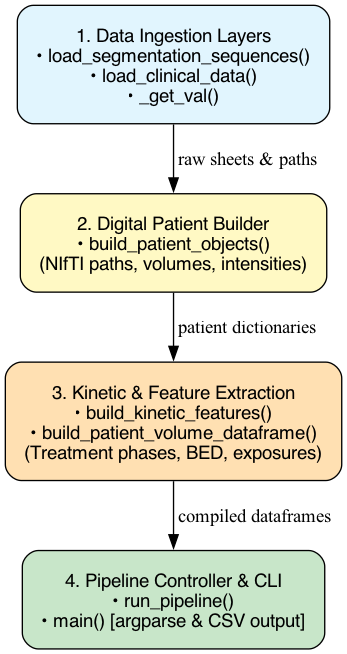
\includegraphics[width=0.35\textwidth]{figures/pipeline_structure.png}
    \caption{Comprehensive pipeline architecture and module interaction flow of the NEXUS Brain Virtual Health Twin (VHT) framework.}
    \label{fig:pipeline_structure}
\end{figure}

The \texttt{vht\_pipeline.py} module implements the core digital patient construction stage of the \textsc{Nexus Brain} VHT framework. It integrates longitudinal MRI derived segmentation and Radiomic measurements with clinical treatment histories to create structured, patient specific datasets for tumor growth calibration, forecasting, and survival analysis. This module produces three main outputs which are integrated patient objects, a longitudinal kinetic feature dataframe, and a volume and exposure dataframe used by the Hierarchical Bayesian Model.

VHT pipeline begins by loading every sheet of the segmentation volume workbook using \texttt{load\_segmentation\_sequences()}. Each sheet corresponds to a tumor subregion or image derived measurement category. It is mapped to a standardized label, such as necrotic core, enhancing tumor, edema, or resection cavity. Module extracts tumor volume, voxel count, and mean and standard deviation intensity values from four MRI sequences for each patient and time point such as contrast enhanced T1-weighted imaging (T1C), non contrast T1-weighted imaging (T1N), T2-FLAIR (T2F), and T2-weighted imaging (T2W). Clinical data are loaded separately using \texttt{load\_clinical\_data()}. Each patient is assigned a cleaned identifier, and the corresponding clinical record is converted into a dictionary containing treatment dates, Radiotherapy dose and fractionation, therapy cycles, molecular biomarkers, and demographic or disease related variables. This structure allows image derived longitudinal measurements and clinical metadata to be joined consistently at the patient level.

The \texttt{build\_patient\_objects()} function integrates the image folder structure, segmentation measurements, and clinical records into a unified patient object. Then pipeline identifies available MRI time points, locates the corresponding NIfTI image files, and attaches segmentation derived volume, voxel, and intensity measurements for each tumor compartment for each patient. These patient objects therefore contain a complete longitudinal representation of those patients, including:

\begin{itemize}
    \item MRI image file paths for every time point
    \item Tumor volumes and voxel counts for necrotic, enhancing, edema, and resection regions
    \item Mean and standard-deviation intensity values across T1C, T1N, T2F, and T2W sequences
    \item Clinical treatment history and molecular biomarkers
    \item A standardized patient identifier linking imaging and clinical data
\end{itemize}

This object oriented structure allows downstream modules to access all patient specific information through a single, consistent data structure. The \texttt{build\_kinetic\_features()} function converts patient objects into a longitudinal dataframe of tumor dynamics and treatment related features. Patients with fewer than two MRI time points are excluded because longitudinal change cannot be calculated without at least two observations. For each time point, the module records the clinical day from diagnosis, compartment specific tumor volumes, and total active tumor volume. Total volume is calculated as the sum of necrotic, enhancing, and edema volumes, while resection cavity volume is retained separately. For every subsequent time point, the pipeline calculates the rate of change of volume, voxel count, MRI intensity, and intratumoral heterogeneity using the elapsed time between scans.

Intensity and heterogeneity changes are computed as weighted combinations of changes across the four MRI sequences. The weights are compartment specific and reflect the expected contribution of each sequence to the biological interpretation of a given tumor region. For example, \texttt{T1C }is weighted more heavily for enhancing tumor, whereas T2-FLAIR and T2-weighted sequences contribute more strongly to edema related features\cite{fan2024radiomics}.

The kinetic dataframe also incorporates treatment timing and Radiobiological information. Each scan is assigned to a treatment phase, pre-treatment, active-treatment, or post-treatment for Chemotherapy, Radiotherapy, additional therapies, Immunotherapy, and Brachytherapy. These phase labels are subsequently converted into dummy encoded indicator variables. Radiotherapy dose and fraction number are used to derive the per fraction dose and the Biological Effective Dose (BED), calculated as:

\begin{equation}
\mathrm{BED}=D\left(1+\frac{d}{\alpha/\beta}\right),
\end{equation}

where $D$ is total prescribed dose, $d$ is dose per fraction, and an $\alpha/\beta$ ratio of 10 Gy is assumed. This feature provides a Radiobiological measure of treatment intensity that can be related to tumor response and survival outcomes. The module also retains treatment cycle length, number of cycles, biological priors, and raw treatment variables. Categorical clinical fields are encoded numerically using label encoding, ensuring that the resulting dataframe can be used directly in statistical and machine-learning models.

The \texttt{build\_patient\_volume\_dataframe()} function creates the primary modeling dataframe used for Bayesian calibration. It retains only patients with at least two longitudinal scans and constructs one row per patient time point.Tt records the patient index, scan day, compartment specific volumes, total tumor volume, core volume, baseline indicator, and inter scan time interval for each row. Treatment exposure is represented as a continuous fraction rather than a simple binary indicator. Pipeline calculates the proportion of time during which a given treatment was active by measuring the overlap between the treatment window and the interval between consecutive scans for each inter scan interval. This approach captures partial treatment exposure and is particularly useful when MRI scans occur during, before, or after an incomplete treatment course. A small overlap threshold is applied to prevent minor timing inconsistencies from incorrectly assigning zero exposure when a treatment window substantially overlaps an imaging interval. The resulting exposure fractions, denoted \texttt{Chemo\_Active}, \texttt{Rad\_Active}, \texttt{Additional1\_Active}, \texttt{Additional2\_Active}, \texttt{Immuno\_Active}, and \texttt{Brachy\_Active}, range from 0 to 1 and are used as time varying treatment covariances in the Fisher-KPP model.

Furthermore, the module computes several derived variables required for tumor growth modeling. Total tumor volume is defined as the sum of necrotic, enhancing, and edema volumes, while core volume is defined as the sum of necrotic and enhancing volumes. The resection cavity volume is retained separately because it represents post surgical anatomy rather than active tumor burden. A patient specific reference carrying capacity, \texttt{Vmax\_Ref}, is calculated as 1.25 times the maximum observed total tumor volume, with a lower bound of 500,000 mm$^3$. This provides an upper bound for the logistic component of the Fisher-KPP growth model and prevents unrealistic unconstrained growth during simulation\cite{rodrigo2021bounds,kostelich2025mathematical}. The inter scan time interval, \texttt{dt}, is calculated for each consecutive pair of scans and is used to estimate tumor volume velocity and treatment exposure. The \texttt{run\_pipeline()} function coordinates the complete workflow. It loads segmentation sequences, loads clinical data, constructs patient objects, extracts kinetic features, and generates the volume and exposure dataframe. The ordering is important because kinetic features are first attached to each patient object and then used to establish reliable scan day mappings in the volume dataframe.

This module is executed as a standalone script or imported into other components of the framework. When run from the command line, it accepts customizable paths for imaging data, segmentation volumes, and clinical records, and can save the kinetic and volume dataframes as \texttt{CSV} files. The modular design supports reproducibility, allows the pipeline to be reused across datasets, and ensures that all downstream modeling components receive consistently structured patient level inputs.



\subsection{Probabilistic Modeling and Parameter Estimation (\texttt{hbm\_Fisher\_kpp.py})}

\begin{figure}[htbp]
    \centering
    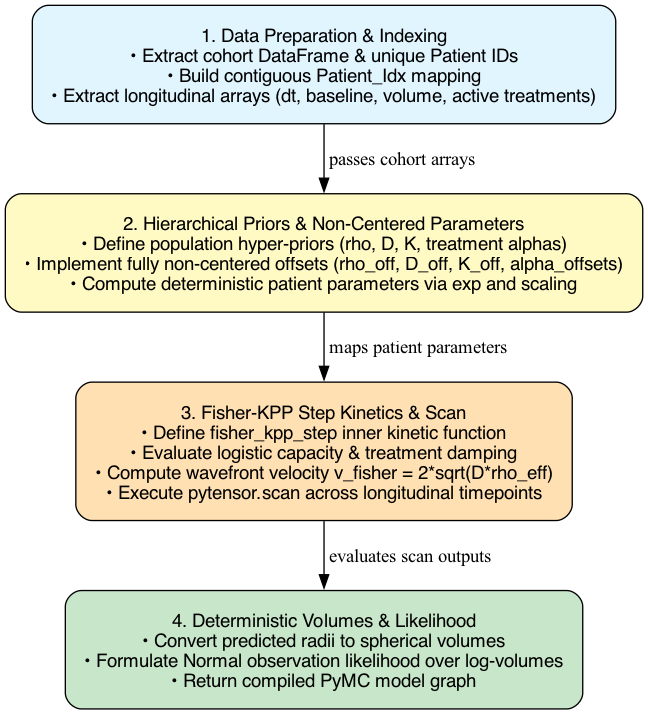
\includegraphics[width=0.35\textwidth]{figures/hbm_structure.png}
    \caption{Comprehensive HBM Fisher--KPP architecture and module interaction flow of the \textsc{Nexus Brain} Virtual Health Twin (VHT) framework.}
    \label{fig:hbm_structure}
\end{figure}

This module implements the Hierarchical Bayesian Model (HBM) used to estimate patient specific Glioblastoma growth and treatment response parameters. It is implemented in \texttt{PyMC} and \texttt{PyTensor} and is based on the Fisher KPP reaction diffusion framework. The model uses longitudinal tumor volume measurements, inter scan time intervals, and treatment exposure fractions to estimate proliferation, diffusion, carrying capacity, and therapy specific inhibitory effects for each patient. The central growth equation is:

\begin{equation}
\frac{\partial c}{\partial t}
=
D\nabla^{2}c
+
\rho c\left(1-\frac{c}{K}\right)
-
\mathrm{Kill}(t)c,
\end{equation}

where $c$ represents tumor cell density, $D$ is the diffusion coefficient, $\rho$ is the proliferation rate, $K$ is the carrying capacity, and $\mathrm{Kill}(t)$ represents treatment induced cell killing or growth inhibition. The module reindexes patients into numeric identifiers by allowing patient specific parameters to be map to every longitudinal observation. It identifies unique patient identifiers and maps each to a integer index beginning at zero. This index is stored in the \texttt{Patient\_Idx} column and aligns patient level parameters with their corresponding longitudinal observations.

The module extracts the following arrays from the cohort dataframe:

\begin{itemize}
    \item Patient index
    \item Inter scan time interval, $\Delta t$
    \item Baseline indicator
    \item Observed total tumor volume
\end{itemize}

It also extracts treatment exposure fractions for Chemotherapy, Radiotherapy, Immunotherapy, two additional systemic-therapy categories, and Brachytherapy. These values range from 0 to 1. They represent the proportion of each inter scan interval during which a treatment was active, allowing the model to account for partial rather than binary exposure. Proliferation, diffusion, and carrying capacity are modeled on the logarithmic scale to ensure strictly positive values and improve numerical stability. For each patient $i$:

\begin{align}
\rho_i &= \exp\left(\mu_{\log \rho}+\sigma_{\log \rho}\epsilon_{\rho,i}\right), \\
D_i &= \exp\left(\mu_{\log D}+\sigma_{\log D}\epsilon_{D,i}\right), \\
K_i &= \exp\left(\mu_{\log K}+\sigma_{\log K}\epsilon_{K,i}\right),
\end{align}

where $\epsilon_{\rho,i}$, $\epsilon_{D,i}$, and $\epsilon_{K,i}$ are patient specific random effects. This non centered parameterization improves sampling efficiency, particularly when the number of patients is moderate and individual level data are limited. Population level means are assigned normal priors, while between patient standard deviations and the observation error standard deviation are assigned half normal priors. Treatment efficacy coefficients use a non centered half normal structure, ensuring non negative effects. Separate coefficients are estimated for Chemotherapy, Radiotherapy, Immunotherapy, two additional systemic therapy categories, and Brachytherapy. Larger coefficients indicate stronger inhibitory effects. The model represents tumor burden using an equivalent spherical radius. At baseline scan of each patient and observed tumor volume is converted into a radius using following equation.

\begin{equation}
r=\left(\frac{3V}{4\pi}\right)^{1/3}.
\end{equation}

This radius is propagated forward through subsequent scan intervals and converted back into an equivalent volume:

\begin{equation}
V=\frac{4}{3}\pi r^{3}.
\end{equation}

This radial formulation allows the Fisher-KPP wavefront approximation to be applied directly to longitudinal volumetric measurements. The model calculates an effective proliferation rate using baseline proliferation, carrying capacity saturation, and treatment mediated inhibition at each longitudinal step. The logistic saturation factor is as follows:

\begin{equation}
1-\frac{V}{K}.
\end{equation}

This factor decreases as tumor volume approaches carrying capacity, reflecting limited growth as the tumor approaches its spatial or biological maximum. A small lower bound is imposed to avoid numerical instability when predicted volume approaches $K$. Treatment inhibition is represented by an exponential damping term:

\begin{equation}
\exp\left(-\sum_{m}\alpha_mE_m\right),
\end{equation}

where $E_m$ is the exposure fraction for treatment $m$. Greater exposure or a larger efficacy coefficient reduces effective proliferation. The effective proliferation rate is therefore:

\begin{equation}
\rho_{\mathrm{eff}}
=
\rho
\left(1-\frac{V}{K}\right)
\exp\left(-\sum_{m}\alpha_mE_m\right).
\end{equation}

The model then uses the Fisher-KPP wavefront velocity approximation:

\begin{equation}
v=2\sqrt{D\rho_{\mathrm{eff}}}.
\end{equation}

The tumor radius is advanced over each inter scan interval as:

\begin{equation}
r_{t+1}=r_t+v\Delta t.
\end{equation}

This produces a predicted tumor volume at each subsequent MRI time point. The recurrence is implemented using \texttt{pytensor.scan}, which sequentially propagates the radius across all patient time observations while retaining the appropriate patient specific parameters and treatment exposures. Then model compares predicted and observed MRI derived total tumor volumes using a normal likelihood on the logarithmic scale. Log transformation is appropriate because tumor volumes are strictly positive, vary over several orders of magnitude, and often exhibit multiplicative rather than additive error structure. The likelihood is:

\begin{equation}
\log V_{\mathrm{obs}}
\sim
\mathcal{N}
\left(
\log V_{\mathrm{pred}},
\sigma_{\log V}
\right),
\end{equation}

where $\sigma_{\log V}$ represents uncertainty from segmentation variability, imaging noise, biological heterogeneity, and model approximation error. A small positive lower bound is applied to predicted and observed volumes before logarithmic transformation to prevent numerical errors from zero or negative values. Bayesian inference simultaneously estimates population level distributions and patient specific proliferation, diffusion, carrying capacity, and treatment efficacy parameters. It allows the framework to borrow strength across the cohort while producing individualized estimates. This \texttt{HBM} forms the calibration core of the \textsc{Nexus Brain} VHT framework. It transforms longitudinal imaging and treatment exposure data into interpretable biological parameters describing tumor proliferation, invasion, carrying capacity constraint, and therapy mediated growth suppression. The estimated parameters are subsequently used in forecasting and counterfactual simulation to project future tumor growth and evaluate alternative treatment strategies. This is how HBM connects longitudinal clinical and imaging data to patient specific virtual twin predictions.



\subsection{\texttt{MCMC} Sampling and Trajectory Plots (\texttt{visualization.py})}

This module provides the cohort level estimation and visualization layer for the Hierarchical Bayesian Model (HBM). It takes patient objects generated by the VHT pipeline and constructs a longitudinal volume and treatment exposure dataframe. Then it fits the Fisher-KPP HBM using Markov chain Monte Carlo (\texttt{MCMC}) to extracts posterior estimates, and generates patient specific growth plots with treatment window shading. Main purpose of this is to connect Bayesian inference with interpretable clinical visualization. It produces trajectory plots showing observed tumor volumes, model-fitted growth curves, and active treatment timing rather than returning only numerical estimates. It also exports \texttt{MCMC} convergence diagnostics, including trace and rank plots, for inspection and reporting. The interaction between data preparation, Bayesian inference, posterior extraction, and visualization is illustrated in Figure~\ref{fig:visualization_structure}.

\begin{figure}[htbp]
    \centering
    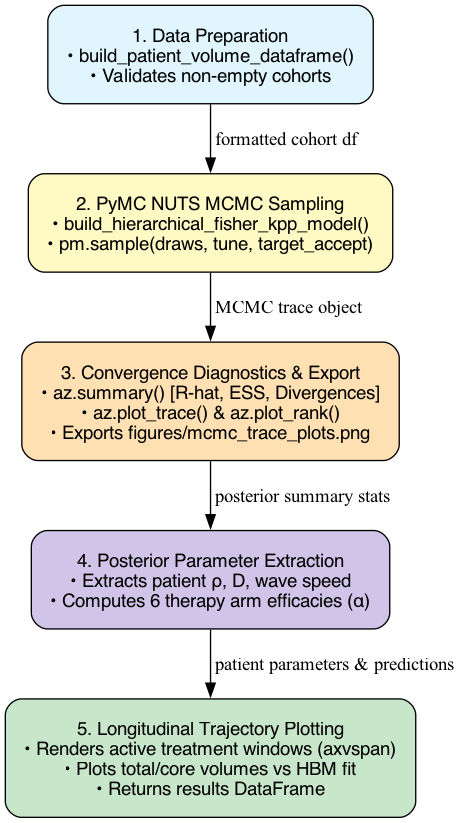
\includegraphics[width=0.35\textwidth]{figures/visualization_structure.png}
    \caption{Comprehensive visualization architecture and module interaction flow of the \textsc{Nexus Brain} Virtual Health Twin (VHT) framework.}
    \label{fig:visualization_structure}
\end{figure}

The function \texttt{estimate\_and\_plot\_each\_patient()} first calls \texttt{build\_patient\_volume\_dataframe()} to convert integrated patient objects into a longitudinal dataframe. This dataframe contains one row per patient time point, including observed total and core tumor volume, scan day, inter scan interval, baseline indicator, and continuous treatment exposure fractions. If the dataframe is empty, the function returns an empty dataframe and terminates without model fitting and prevents application of the HBM to invalid or insufficient input. Patients with fewer than two longitudinal scans are excluded during dataframe construction because tumor growth dynamics cannot be estimated from repeated measurements. The resulting dataframe is passed to \texttt{build\_hierarchical\_fisher\_kpp\_model()}, which constructs the \texttt{PyMC} model graph for all patients simultaneously. The number of unique patients is determined from the \texttt{Patient\_Idx} column, and the cohort level model is initialized accordingly.

The HBM is fitted using the No-U-Turn Sampler (\texttt{NUTS}) in \texttt{PyMC}, a Hamiltonian Monte Carlo method designed for efficient sampling from high dimensional posterior distributions. The sampler is configured with 2,000 tuning steps and 1,000 posterior draws. The tuning phase allows adaptation of the step size and mass matrix before formal posterior samples are collected. A target acceptance probability of 0.99 is specified to reduce divergent transitions and improve sampling stability. A fixed random seed of 42 promotes reproducibility across repeated executions. Because all patients are modeled jointly, inference estimates both population level hyperparameters and patient specific growth parameters, allowing information sharing across the cohort while producing individualized estimates.

Then module uses \texttt{ArviZ} to generate convergence diagnostics for the population level hyperparameters \texttt{mu\_log\_rho}, \texttt{mu\_log\_D}, \texttt{mu\_log\_K}, and the observation error standard deviation \texttt{sigma\_obs\_log\_v}. For each parameter, the posterior mean, standard deviation, split-$\widehat{R}$ statistic, Bulk Effective Sample size (\texttt{ess\_bulk}), and tail effective sample size (\texttt{ess\_tail}) are reported. The module also counts divergent transitions in \texttt{trace.sample\_stats.diverging}, which indicate regions where the Hamiltonian Monte Carlo sampler may fail to explore the posterior reliably. Multi chain trace plots for the population level hyperparameters are saved as \texttt{figures/mcmc\_trace\_plots.png}, and rank plots are saved as \texttt{figures/mcmc\_rank\_plots.png}. Trace plots assess chain stationarity and mixing, while rank plots assess overlap of rank distributions across independent chains. These diagnostics provide an initial assessment of sampler behavior. Formal convergence assessment also consider numerical $\widehat{R}$, ESS, and divergence count thresholds.

Following the sampling, the module uses ArviZ to summarize posterior distributions. Population level summaries are reported for the logarithmic means of proliferation, diffusion, and carrying capacity, as well as the observation error standard deviation. The posterior mean, standard deviation, and 94\% Highest Density Interval (HDI) are extracted for each parameter. The HDI represents the narrowest interval containing the specified proportion of posterior probability mass and provides an uncertainty range for each estimated parameter. The module also extracts the posterior mean predicted tumor volume trajectory, \texttt{pred\_volumes}, directly from the \texttt{PyMC} trace, representing the model fitted growth curve for each patient across observed MRI time points. The module extracts posterior mean estimates of proliferation ($\rho$), diffusion ($D$), and treatment-efficacy coefficients ($\alpha_m$) for every patient. The Fisher-KPP wavefront speed is calculated as follows:

\begin{equation}
v = 2\sqrt{D\rho}.
\end{equation}

If a wavefront speed variable is available in the posterior summary, it is retrieved from the trace. Otherwise, it is computed from posterior mean estimates of $D$ and $\rho$. Treatment effects are converted into interpretable deceleration factors using:

\begin{equation}
\mathrm{Effect}_m = e^{-\alpha_m},
\end{equation}

where $\alpha_m$ is the posterior mean efficacy coefficient for treatment $m$. The corresponding percentage reduction in effective proliferation is:

\begin{equation}
\mathrm{Reduction}_m = \left(1 - e^{-\alpha_m}\right) \times 100\%.
\end{equation}

For example, an efficacy coefficient of $\alpha = 0.5$ corresponds to an approximate 39.3\% reduction in effective proliferation during active exposure. The module evaluates treatment specific effects for Chemotherapy, Radiotherapy, two additional systemic therapy categories, Immunotherapy, and Brachytherapy. The corresponding effect is recorded as not modeled if a treatment specific efficacy parameter is unavailable in the posterior summary. The module generates a longitudinal plot showing observed and modeled tumor dynamics for each patient. Total tumor volume is plotted as a black line with circular markers, while core volume, defined as the sum of necrotic and enhancing volumes, is plotted separately where available. The posterior mean HBM trajectory is overlaid in red, representing fitted tumor volume predictions across observed scan days and enabling visual assessment of model fit. The trajectory is plotted only when the number of extracted posterior row indices matches the number of longitudinal observations for that patient. Treatment windows are shaded in the background, with distinct colors for Chemotherapy, Radiotherapy, additional systemic therapies, Immunotherapy, and Brachytherapy. Start and End days are extracted from clinical record of the patient, and shaded regions indicate active treatment. If an end date is unavailable, the window is extended to the latest available scan day. If the end date is earlier than or equal to the start date, a nominal two day window is used to ensure visibility.

These plots allow qualitative assessment of the relationship between treatment timing and tumor volume trajectory. For example, reduced volume or slowed growth during a shaded Radiotherapy window may be consistent with a treatment mediated inhibitory effect, whereas continued growth despite exposure may indicate limited efficacy, incomplete exposure, or model limitations. The visual layer complements numerical posterior estimates by making patient specific model behavior transparent, enabling inspection of whether the HBM captures observed tumor kinetics and whether estimated treatment effects are plausible in the clinical context. The function returns a dataframe with one row per patient containing posterior mean estimates of:

\begin{itemize}
    \item Proliferation rate, $\rho$
    \item Diffusion coefficient, $D$
    \item Fisher--KPP wavefront speed
    \item Treatment-specific efficacy coefficients
    \item Derived treatment-effect percentages
\end{itemize}

These patient level estimates can be used for cohort level analysis, biomarker association studies, counterfactual forecasting, and survival modeling. This module utilize the HBM as an end to end estimation and interpretation workflow, linking longitudinal tumor volume data, treatment exposure, Bayesian inference, convergence diagnostics, and clinical visualization. It supports evaluation of model fit, treatment response estimation, and identification of individual variation in Glioblastoma growth dynamics by producing both posterior parameter estimates and interpretable patient specific trajectory plots. The exported trace and rank plots further support transparent reporting of \texttt{MCMC} behavior and provide a reproducible visual record of posterior sampling quality.



\subsection{Forecasting and Counterfactual Simulation (\texttt{vht\_forecast.py})}

\begin{figure}[htbp]
    \centering
    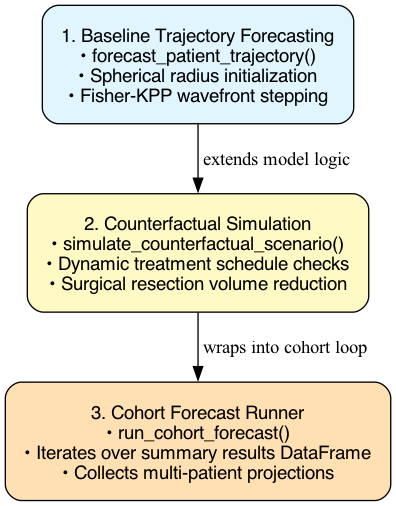
\includegraphics[width=0.35\textwidth]{figures/forecast_structure.png}
    \caption{Comprehensive forecast architecture and module interaction flow of the NEXUS Brain Virtual Health Twin (VHT) framework.}
    \label{fig:forecast_structure}
\end{figure}

This module implements the predictive forecasting and counterfactual simulation component of the \textsc{NEXUS Brain} VHT framework. As mentioned earlier it uses patient specific parameters estimated by the Hierarchical Bayesian Model to project future Glioblastoma tumor growth beyond the last available MRI time point. The module supports a baseline forecast under continued or absent treatment and dynamic "what-if" counterfactual scenarios in which future treatments or surgical resections are introduced at specified times. The forecasting engine is based on the Fisher-KPP reaction diffusion wavefront approximation. It converts the last observed tumor volume into an equivalent spherical radius, advances that radius forward using patient specific proliferation and diffusion parameters, and converts the simulated radius back into tumor volume. The function \texttt{forecast\_patient\_trajectory()} generates a forward tumor growth projection for an individual patient. It begins with the last observed total tumor volume, converts it into an equivalent spherical radius using:

\begin{equation}
r = \left(\frac{3V}{4\pi}\right)^{1/3}.
\end{equation}

At each daily simulation step, the current radius is converted back into an equivalent tumor volume:

\begin{equation}
V = \frac{4}{3}\pi r^3.
\end{equation}

The model then applies a carrying capacity saturation factor:

\begin{equation}
1 - \frac{V}{K},
\end{equation}

where $K$ is the patient specific carrying capacity. This factor slows growth as simulated tumor volume approaches its estimated maximum sustainable burden. Treatment effects are incorporated through an exponential damping term. For each therapy $m$, the product of its efficacy coefficient $\alpha_m$ and active flag contributes to the total inhibitory effect. The effective proliferation rate is therefore:

\begin{equation}
\rho_{\text{eff}} = \rho \left(1 - \frac{V}{K}\right) \exp\left(-\sum_m \alpha_m A_m\right),
\end{equation}

where $A_m$ is the active treatment flag. The Fisher-KPP wavefront velocity is then calculated as:

\begin{equation}
v = 2\sqrt{D\rho_{\text{eff}}},
\end{equation}

and the tumor radius is advanced by:

\begin{equation}
r_{t+1} = r_t + v\Delta t.
\end{equation}

The output is a dataframe containing forecast day, relative to the last observed scan, and the corresponding predicted tumor volume. The function \texttt{simulate\_counterfactual\_scenario()} extends the baseline forecast by allowing dynamic interventions at specified future calendar days. This enables evaluation of hypothetical treatment strategies not necessarily observed in the patient’s actual clinical course. Treatment schedules are defined as a list of interventions, each specifying treatment type, start day, end day, and activity level. During simulation, the module checks whether the current forecast day falls within each treatment window. If it does, the corresponding calibrated efficacy coefficient is applied to reduce effective proliferation. This allows simulation of scenarios such as:

\begin{itemize}
    \item Starting Chemotherapy after the last observed scan
    \item Extending or delaying Radiotherapy
    \item Adding Immunotherapy or Brachytherapy
    \item Combining multiple treatment modalities
    \item Comparing treatment versus no treatment trajectories
\end{itemize}

Treatment exposure is evaluated dynamically at every simulation step, allowing therapies to begin, end, or overlap during the forecast horizon unlike the baseline forecast. The counterfactual module also supports virtual surgical resection events. A resection is specified by a future day and a volume reduction fraction. When the simulation reaches the specified resection day, the current modeled tumor volume is reduced by the defined proportion:

\begin{equation}
V_{\text{post}} = V_{\text{pre}}(1 - f),
\end{equation}

where $f$ is the resection fraction. The equivalent spherical radius is then recalculated from the reduced volume, and tumor growth continues from this post resection state. For example, an $80\%$ resection reduces simulated tumor volume to $20\%$ of its pre resection value. The model then projects regrowth from this reduced burden using the calibrated proliferation, diffusion, and carrying capacity parameters of patient. This enables evaluation of hypothetical surgical timing and extent on future tumor burden.

The function \texttt{run\_cohort\_forecast()} applies the baseline forecasting procedure across all patients with calibrated HBM parameters. It retrieves posterior mean estimates of proliferation, diffusion, carrying capacity, and treatment efficacy coefficients from the model results dataframe for each patient. Then module identifies the final observed MRI time point and uses its day and total tumor volume as the starting condition for forecasting. After that it generates a forward projection over a specified horizon, defaulting to $180$ days. Patients without available longitudinal volume data are excluded. The result is a dictionary mapping each patient identifier to a dataframe of forecast days and predicted tumor volumes. These cohort level projections can be used for comparative analysis, identification of patients predicted to experience rapid progression, and downstream survival or risk stratification analyses.

Overall this module translates calibrated tumor growth parameters into clinically interpretable future predictions. It connects Bayesian calibration to practical decision support by allowing users to project tumor burden under observed treatment conditions and compare it with hypothetical alternatives. The framework supports counterfactual evaluation of multimodal treatment planning by combining patient specific proliferation, diffusion, carrying capacity, treatment efficacy, and virtual resection events. This enables exploration of how the timing of Chemotherapy or Radiotherapy, addition of Immunotherapy, or extent and timing of surgical resection may alter projected tumor growth beyond the last clinical observation.



\subsection{Survival Modeling (\texttt{cox\_survival\_ht.py})}

\begin{figure}[htbp]
    \centering
    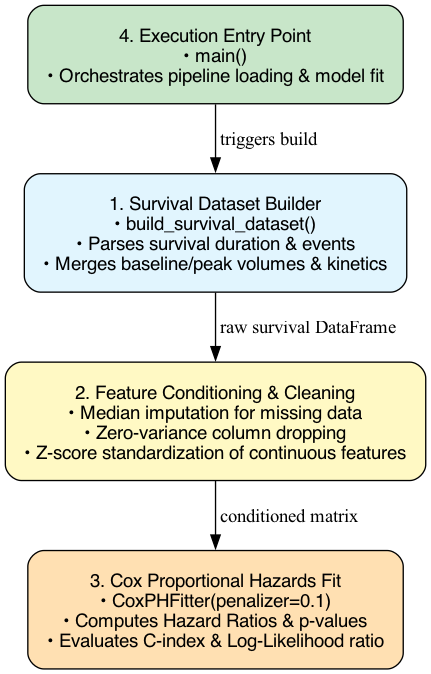
\includegraphics[width=0.35\textwidth]{figures/cox_structure.png}
    \caption{Comprehensive cox model architecture and module interaction flow of the NEXUS Brain Virtual Health Twin (VHT) framework.}
    \label{fig:cox_structure}
\end{figure}

This module links tumor dynamics features generated by the \textsc{NEXUS Brain} VHT pipeline to patient survival outcomes using Cox proportional hazards regression. It constructs a patient level survival dataset from longitudinal imaging, kinetic, and clinical data. Then it fits a regularized Cox model to estimate associations between baseline tumor burden, tumor growth velocity, age, molecular biomarkers, and overall survival. The module uses the \texttt{lifelines} implementation of the Cox proportional hazards model. Its primary output is a set of hazard ratios, confidence intervals, and p-values describing how each covariance is associated with the risk of death, together with a concordance index measuring predictive discrimination.

The function \texttt{build\_survival\_dataset()} converts patient objects, the longitudinal volume dataframe, and the kinetic feature dataframe into one row per patient. It extracts survival duration and event indicator from the clinical record. Survival duration is obtained from clinical fields representing days from diagnosis to death, overall survival in days, survival time, or days to death or last follow up. The module uses the latest imaging day of patient as a censored follow up time if no valid survival duration is available. Although it should be interpreted as a conservative fallback rather than a true survival endpoint, this prevents patients with missing survival data from being discarded entirely. The event indicator is derived from an explicit death field when available. If absent, vital status text is parsed for terms indicating death, such as “dead,” “deceased,” or “expired.” Patients without evidence of death are treated as censored observations which means their exact survival time is unknown but they were known to be alive at last follow up.

The survival dataset includes image derived covariances representing tumor burden and growth dynamics. Baseline total and enhancing tumor volumes are taken from the first available MRI time point. Peak total tumor volume is defined as the maximum observed total volume across all available scans. The module also calculates mean enhancing tumor velocity from the kinetic feature dataframe. Also it represents the average rate of change in enhancing tumor volume over time and capturing longitudinal growth or shrinkage of contrast enhancing disease. This variable allows the survival model to assess whether dynamic tumor behavior adds prognostic information beyond static baseline volume measurements. Patient age is extracted from available clinical fields and included as a standard clinical covariance. Missing age values are imputed using the cohort median, with a fallback value of 60 years if no valid median can be calculated.

This module incorporates established Glioblastoma molecular and genetic biomarkers, including \texttt{IDH1} mutation, \texttt{MGMT} Methylation, and \texttt{1p/19q} codeletion. These variables are added to the survival dataset from clinical record of each patient. Missing biomarker values are imputed as zero, and categorical variables are converted to numeric form using label encoding. This ensures the Cox model receives a complete, numerically encoded feature matrix. Module performs preprocessing steps to improve numerical stability and prevent overfitting before fitting the Cox model. Missing continuous covariances are imputed using cohort medians. Rows with missing survival duration or event status are removed because these fields are required for survival analysis. Constant features with zero variance are excluded, since they provide no information for distinguishing patients and can cause numerical instability during model fitting. Continuous covariances are then standardized by subtracting the mean and dividing by the standard deviation. Standardization places all continuous variables on a comparable scale and reduces the risk of ill conditioned optimization. Then Cox proportional hazards model estimates the relationship between covariances and the hazard of death. The model assumes that the hazard for patient $i$ is:

\begin{equation}
h_i(t) = h_0(t)\exp(\beta_1x_{i1} + \beta_2x_{i2} + \cdots + \beta_px_{ip}),
\end{equation}

where $h_0(t)$ is the baseline hazard, $x_{ij}$ are patient covariances, and $\beta_j$ are regression coefficients. A positive coefficient indicates that higher values of the covariance are associated with increased mortality risk, whereas a negative coefficient indicates a protective association. The model is fitted with an $L_2$ penalization term of 0.1. Regularization shrinks coefficient estimates and reduces overfitting, which is particularly important when the number of covariances is large relative to the number of patients or when predictors are correlated. The fitted model reports regression coefficients, exponentiated coefficients, standard errors, p-values, and 95\% confidence intervals. The exponentiated coefficient is the hazard ratio (HR):

\begin{equation}
\text{HR} = e^{\beta}.
\end{equation}

An Hazard Ratio(HR) greater than 1 indicates that a one standard deviation increase in the standardized covariance is associated with higher mortality risk. An HR less than 1 indicates a lower associated risk. The concordance index (\texttt{C-index}) is reported as a measure of discriminatory performance, representing the probability that, for a randomly selected pair of patients. The patient with the shorter observed survival time has the higher predicted risk. A C-index of 0.5 indicates performance no better than chance, while a value closer to 1 indicates stronger discrimination. The likelihood ratio test evaluates whether the fitted model provides a statistically significant improvement over a null model containing no covariances. A small p-value suggests that the included clinical, imaging, kinetic, or biomarker features collectively contribute prognostic information.

This module completes the \textsc{NEXUS Brain} VHT framework by connecting model derived tumor kinetics and imaging features to clinical outcomes. It evaluates whether baseline tumor burden, enhancing tumor growth velocity, age, and molecular biomarkers are associated with overall survival. The analysis tests whether the virtual health twin captures prognostically relevant biological variation beyond conventional clinical and molecular predictors by incorporating longitudinal imaging derived features into a regularized survival model. The resulting hazard ratios and concordance index provide a quantitative assessment of the clinical relevance of the framework’s tumor-dynamics features.



\subsection{Interactive Dashboard (\texttt{vht\_dashboard.py})}

\begin{figure}[htbp]
    \centering
    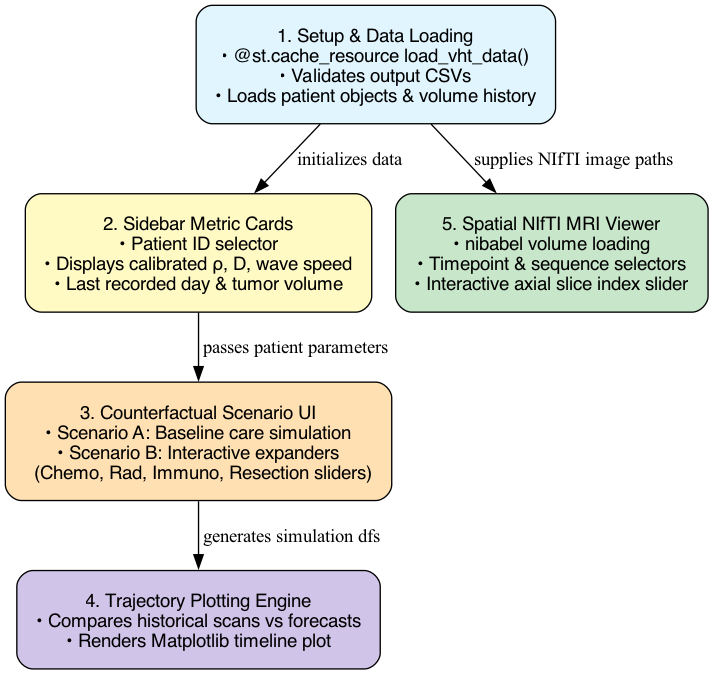
\includegraphics[width=0.45\textwidth]{figures/dashboard_structure.png}
    \caption{Comprehensive dashboard architecture and module interaction flow of the NEXUS Brain Virtual Health Twin (VHT) framework.}
    \label{fig:dashboard_structure}
\end{figure}

This module implements the interactive clinical exploration layer of the \textsc{NEXUS Brain} VHT framework. It is a \texttt{Streamlit}-based dashboard that allows users to select an individual patient, inspect calibrated tumor growth parameters, simulate counterfactual treatment and surgical scenarios, visualize projected tumor volume trajectories, and review longitudinal MRI scans. The dashboard connects the previously described data processing, Bayesian calibration, and forecasting modules into a single interactive interface. Its purpose is to translate patient specific model outputs into an accessible visual tool for exploring “what-if” clinical decisions.

Upon launch, the dashboard loads the calibrated HBM parameter summary and longitudinal volume history files generated by the main pipeline. It also loads integrated patient objects containing MRI file paths, tumor volumes, Radiomic measurements, and clinical metadata. The user selects a patient from a sidebar dropdown menu. Once selected, the dashboard retrieves the calibrated proliferation rate ($\rho$), diffusion coefficient ($D$), Fisher-KPP wavefront speed, last recorded scan day, and last observed total tumor volume of patient. These values are displayed as sidebar metric cards. It provides an immediate summary of estimated tumor growth phenotype of the patient. The dashboard also extracts calibrated treatment efficacy coefficients for Chemotherapy, Radiotherapy, Immunotherapy, additional systemic therapies, and Brachytherapy. These coefficients determine how strongly each therapy suppresses effective proliferation during counterfactual simulation.

The dashboard compares two future growth scenarios over a 180-day forecast horizon. Scenario A represents a baseline projection with no additional therapy. It uses thelast observed tumor volume of patient as the starting condition and applies calibrated proliferation, diffusion, and carrying capacity parameters to simulate future growth under the Fisher-KPP wavefront model. Scenario B represents a customized counterfactual multimodal intervention. The user can configure hypothetical Chemotherapy, Radiotherapy, Immunotherapy, Brachytherapy, and surgical resection using interactive controls. For drug or Radiation based therapies, the user specifies a start day and end day. For surgical resection, the user specifies the day of surgery and the percentage of tumor volume to be removed. The counterfactual simulation dynamically evaluates whether each treatment is active on each simulated day. When a therapy is active when a resection event occurs. Its calibrated efficacy coefficient reduces effective proliferation. The simulated tumor volume is instantaneously reduced by the selected percentage, and subsequent growth continues from the post resection volume.

The dashboard generates a longitudinal plot comparing historical observations with the two simulated futures. Historical MRI derived total tumor volumes are plotted as black points connected by a line, showing the observed disease course up of patient to the last available scan. Scenario A is plotted as a dashed red line, representing projected tumor growth without additional intervention. Scenario B is plotted as a green line, representing projected tumor burden under the user defined counterfactual treatment strategy. This visualization allows direct comparison between the baseline forecast and the simulated intervention. For example, the user can assess whether earlier Chemotherapy, extended Radiotherapy, addition of Immunotherapy, or surgical resection is projected to reduce tumor volume relative to the no treatment scenario.

The dashboard also includes a spatial MRI and tumor evolution viewer. The user can choose an available MRI time point and then select a specific \texttt{NIfTI} file for the selected patient, such as an anatomical sequence or segmentation mask. The selected \texttt{NIfTI} volume is loaded using \texttt{nibabel}, and an axial slice is displayed using \texttt{Matplotlib}. The user can navigate through the image volume using an axial slice slider. The displayed image is rotated by 90 degrees for conventional radiological visualization and rendered in grayscale. This component allows users to inspect the spatial imaging data underlying longitudinal volumetric measurements. It provides visual context for model inputs by enabling review of tumor appearance, segmentation related structures, and changes across MRI time points. This dashboard serves as the translational interface of the \textsc{NEXUS Brain} VHT framework. It converts patient specific HBM parameters and Fisher-KPP simulations into an interactive environment for exploring hypothetical clinical decisions. By combining calibrated growth parameters, treatment efficacy estimates, counterfactual forecasting, and MRI visualization, the module supports patient specific scenario analysis. It enables users to evaluate how alternative treatment timing, treatment combinations, or surgical resection strategies may alter projected



\subsection{Main Execution Script (\texttt{main.py})}

\begin{figure}[htbp]
    \centering
    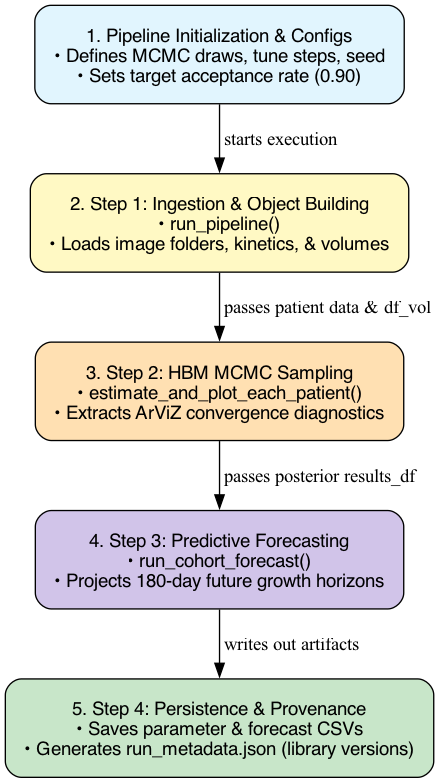
\includegraphics[width=0.34\textwidth]{figures/main_structure.png}
    \caption{Comprehensive main architecture and module interaction flow of the NEXUS Brain Virtual Health Twin (VHT) framework.}
    \label{fig:main_structure}
\end{figure}

The main execution script orchestrates the complete \textsc{NEXUS Brain} VHT workflow. It coordinates data ingestion, digital patient construction, Hierarchical Bayesian Model (HBM) parameter estimation, cohort visualization, predictive forecasting, and persistence of primary outputs. The script ensures each analytical stage receives the correct inputs in the required order by executing the pipeline as a single controlled workflow. It produces a reproducible end to end analysis, beginning with raw segmentation and clinical data and ending with calibrated patient parameters, forecasted tumor growth trajectories, and a machine readable provenance record.

In the first stage, the script calls \texttt{run\_pipeline()} from \texttt{vht\_pipeline.py}. This loads longitudinal MRI derived segmentation and Radiomic sequences, clinical treatment histories, and molecular biomarkers. Then it constructs integrated patient objects and generates two structured dataframes of a kinetic feature dataframe and a volume and exposure dataframe. The kinetic dataframe contains longitudinal tumor volume changes, growth velocities, image derived intensity and heterogeneity changes, treatment phases, Radiobiological features, and biomarker variables. The volume and exposure dataframe contains patient level longitudinal tumor volumes, scan days, inter scan intervals, and continuous treatment exposure fractions. These outputs form the inputs required for Bayesian calibration. Before proceeding, the script checks whether the volume dataframe is empty. If no valid longitudinal volume data are available, execution stops with an error message, preventing downstream modeling on incomplete inputs.

In the second stage, the script invokes \texttt{estimate\_and\_plot\_each\_patient()} to fit the Fisher-KPP Hierarchical Bayesian Model. This function constructs the \texttt{PyMC} model, performs \texttt{MCMC} sampling, extracts posterior summaries, and generates patient specific longitudinal trajectory plots. \texttt{PyMC} settings are explicitly defined for reproducibility. The current configuration uses 1000 posterior draws and 2000 tuning steps, with a target acceptance probability of 0.99 and a random seed of 42. These settings are intended for rapid testing and pipeline validation. The output of this stage is a patient level results dataframe containing posterior mean estimates of proliferation ($\rho$), diffusion ($D$), wavefront speed, and treatment efficacy coefficients for Chemotherapy, Radiotherapy, Immunotherapy, additional therapies, and Brachytherapy.

In the third stage, the script runs the cohort level forecasting engine using \texttt{run\_cohort\_forecast()}. For each patient with valid calibrated parameters and longitudinal volume history, the module generates a 180-day forward projection of tumor growth. The forecast initializes from most recently observed tumor volume of each patient and uses their posterior mean proliferation, diffusion, carrying capacity, and treatment efficacy estimates. The resulting trajectories represent expected future tumor burden under the calibrated Fisher-KPP growth model. These forecasts provide a cohort level view of predicted disease progression and serve as the basis for subsequent counterfactual simulations in the interactive dashboard.

In the final stage, the script saves all primary analytical outputs to an \texttt{output/} directory. The HBM posterior parameter summary is saved as \texttt{hbm\_patient\_parameters\_summary.csv}, containing one row per patient with calibrated growth and treatment response parameters required by the forecasting and dashboard modules. Cohort forecasts are combined into a single dataframe and saved as \texttt{vht\_tumor\_growth\_forecasts.csv}. The longitudinal volume and exposure dataframe is saved as \texttt{df\_vol.csv}, preserving the observed tumor volume history and treatment exposure features used for model calibration. These persisted outputs allow the dashboard and downstream analyses to reload calibrated results without repeating the computationally expensive \texttt{MCMC} procedure.

The script also generates a provenance metadata file, \texttt{run\_metadata.json}, recording the execution timestamp, cohort size, software-library versions, and \texttt{MCMC} configuration, including the number of draws, tuning steps, target acceptance probability, and random seed. This provenance log supports reproducibility by documenting the computational environment and analytical settings used to generate results. It enables future users to determine whether outputs were produced under the same software versions and sampling configuration, and provides an audit trail connecting result files to a specific pipeline execution.

The main execution script functions as the computational controller of the \textsc{NEXUS Brain} VHT framework. It links data ingestion, feature extraction, Bayesian calibration, visualization, and predictive forecasting into a single reproducible workflow. The script ensures patient specific virtual health twins are generated consistently from raw clinical and imaging data by standardizing execution order and persisting intermediate and final outputs. Its provenance logging further supports transparency, reproducibility, and traceability across the full modeling pipeline.


\subsection{Testing and Verification Architecture}

\begin{figure}[htbp]
    \centering
    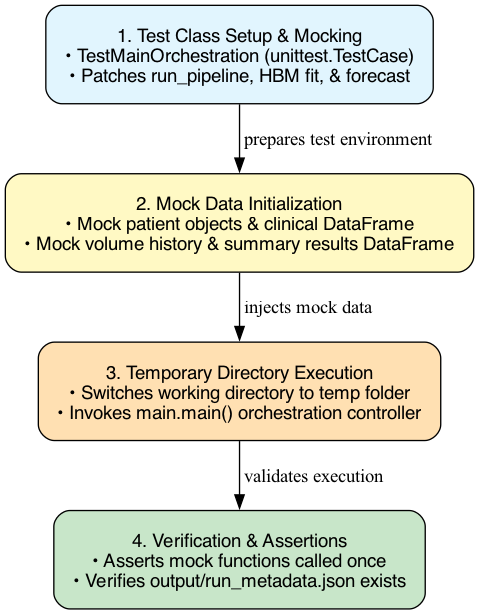
\includegraphics[width=0.35\textwidth]{figures/test_main_structure.png}
    \caption{Comprehensive test architecture and module interaction flow of the NEXUS Brain Virtual Health Twin (VHT) framework.}
    \label{fig:test_structure}
\end{figure}

The testing and verification architecture of the \textsc{Nexus Brain} VHT framework is organized into five core layers. Together, these layers provide a structured quality assurance workflow that evaluates data integrity, feature engineering correctness, Bayesian model construction, forecasting functionality, and end to end pipeline orchestration. The purpose is to identify implementation errors before they propagate into downstream Bayesian calibration, counterfactual simulation, or survival modeling.

The first layer, implemented in \texttt{test\_vht\_helper\_functions.py} and \texttt{test\_vht\_pipeline.py}, validates individual helper functions and feature extraction algorithms using isolated test inputs and synthetic patient objects. This layer verifies that the mathematical and data-processing operations underlying the VHT framework produce expected outputs. Tests evaluate string and numeric parsing, ensuring heterogeneous clinical fields can be safely converted to numerical values. For example, a dose recorded as “60 Gy” or a fraction count recorded as “30 fractions” should be correctly parsed as 60.0 and 30.0, respectively. Missing, malformed, or non numeric values are handled explicitly and returned as \texttt{NaN}, preventing invalid values from entering downstream models. Tests also validate kinetic metrics, including volumetric velocity, total tumor volume, and core tumor volume. Total tumor volume is calculated as the sum of necrotic, enhancing, and edema volumes, while core volume is the sum of necrotic and enhancing volumes. Resection cavity volume is excluded from total tumor burden because it represents post surgical anatomy rather than active tumor tissue. Radiobiological calculations are verified using the linear quadratic Biological Effective Dose (BED) formulation. Tests confirm that total radiation dose, number of fractions, per fraction dose, and BED are calculated correctly according to specified Radiobiological assumptions. Finally, tests validate treatment overlap fractions. For each inter scan interval, the framework calculates the proportion of time a treatment was active. Tests confirm these exposure fractions remain bounded between 0 and 1 and correctly reflect overlap between treatment start and end dates and the interval between consecutive MRI scans.

The second test layer, implemented in \texttt{test\_hbm\_Fisher\_kpp.py}, evaluates the structural integrity, tensor dimensionality, and \texttt{MCMC} readiness of the \texttt{PyMC} and PyTensor Fisher-KPP model graph. This layer ensures the Hierarchical Bayesian Model can be constructed correctly before full scale posterior inference. Model construction tests confirm that \texttt{build\_hierarchical\_fisher\_kpp\_model()} returns a valid \texttt{PyMC} model instance and contains required population level hyperpriors, including $\mu_{\log \rho}$, $\mu_{\log D}$, and $\mu_{\log K}$. They also verify the presence of deterministic patient specific parameters, including proliferation, diffusion, carrying capacity, and predicted tumor volume trajectories. Tensor dimension tests ensure patient level parameter arrays match the number of unique patients in the cohort. For example, proliferation and treatment efficacy arrays must have one element per patient, while predicted volume tensors must have one element per patient time point observation. These checks prevent dimension mismatches that could otherwise cause model construction or sampling errors. The test suite also performs rapid multi chain smoke sampling to verify that \texttt{MCMC} diagnostics can be generated. It checks that \texttt{ArviZ} produces convergence metrics, including split R-hat ($\widehat{R}$) and bulk effective sample size (\texttt{ess\_bulk}), and tracks divergent transitions. These diagnostics provide an initial assessment of sampler behavior.

The third test layer, implemented in \texttt{test\_vht\_forecast.py} and \texttt{test\_vht\_dashboard.py}, validates prospective forecasting routines and interactive dashboard logic. This layer ensures calibrated patient specific parameters can be translated into future tumor growth projections and counterfactual clinical scenarios. Scenario A tests baseline forecasting by generating unconstrained forward growth projections from last recorded MRI scan of each patient. These projections use calibrated proliferation and diffusion parameters while accounting for carrying capacity saturation and treatment mediated inhibition. Scenario B tests counterfactual simulations involving complex multimodal treatment schedules. Tests verify that overlapping Chemotherapy, Radiotherapy, Immunotherapy, and Brachytherapy windows can be incorporated into a single simulation. They also validate instantaneous surgical volume reductions, where a specified fraction of tumor volume is removed at a defined future time point. Cohort batch processing tests evaluate the forecasting ability of engine to generate projections across multiple patient profiles. And it confirms that the framework can scale from individual patient simulation to cohort level analysis and enabling identification of patients predicted to experience rapid progression.

The fourth test layer, implemented in \texttt{test\_main.py} and \texttt{test\_visualization.py}, ensures end to end execution flow, robust error handling, and correct integration between pipeline components. This layer verifies that the main execution script correctly links data ingestion, HBM parameter fitting, cohort forecasting, and provenance metadata generation. Using \texttt{unittest.mock}, tests simulate execution of \texttt{main.py} and verify each stage is invoked in the correct sequence. They also confirm the pipeline generates and saves required outputs, including posterior parameter summaries, forecast files, longitudinal volume history, and the \texttt{run\_metadata.json} provenance log. Visualization tests evaluate the robustness of \texttt{estimate\_and\_plot\_each\_patient()}. Using mocked \texttt{MCMC} sampling and plotting routines, tests verify the function can process valid mock patient structures, extract posterior summaries, calculate treatment effect estimates, and generate longitudinal trajectory plots. Tests also assess graceful error handling. The visualization function detects the absence of usable longitudinal data, issues a diagnostic warning, and exits without attempting \texttt{MCMC} inference when the volume dataframe construction step returns an empty dataframe. This prevents silent failures and ensures the pipeline does not produce misleading results from insufficient input data.

The fifth test layer, implemented in \texttt{test\_cox\_data\_integrity.py}, acts as an automated data hygiene check prior to advanced survival analysis and statistical modeling. Its purpose is to ensure the survival dataset and feature matrix are numerically valid and suitable for Cox proportional hazards regression. This layer queries pipeline outputs and inspects survival related datasets for corrupted or invalid values. Specifically, it checks for missing values (\texttt{NaN}), infinite values (\texttt{Inf}), and zero variance features that provide no discriminatory information. These checks apply to key clinical and image derived covariates, including baseline tumor volume, enhancing tumor velocity, patient age, \textit{IDH1} mutation status, \texttt{MGMT} Methylation status, and \texttt{1p/19q} codeletion status. This layer reduces the risk of numerical instability, ill-conditioned optimization, and invalid coefficient estimation by identifying missing, infinite, or constant features before model fitting. It also ensures the Cox model receives a complete and interpretable feature matrix.

Together, these five test layers provide a comprehensive verification architecture for the \textsc{Nexus Brain} VHT framework. They evaluate the framework at multiple levels, from individual helper functions to full end to end pipeline orchestration. This layered approach separates different types of assurance. Data integrity tests verify inputs are suitable for modeling. Unit tests verify feature engineering calculations are mathematically correct. HBM tests verify the Bayesian model is structurally valid. Forecasting tests verify calibrated parameters can be translated into future projections. And orchestration tests verify the complete workflow executes reliably.

